\section{Processi primari}
	\subsection{Fornitura}
		\subsubsection{Introduzione processo}
			\paragraph{Descrizione}
				Il processo di fornitura viene svolto dal gruppo EverBuilds per capire e comprendere le richieste del proponente al fine di diventare fornitori per l’azienda Zero12 e per i Committenti prof. Tullio Vardanega e prof. Riccardo Cardin. Ogni membro del gruppo è tenuto, durante tutte le fasi di progettazione, sviluppo e consegna del prodotto, ad attenersi a quanto esposto nel documento.\\
			\paragraph{Obbiettivi}
				L’obiettivo è quello di formalizzare le norme e le procedure che dovranno poi essere applicate dal gruppo EverBuilds. Per fare ciò il gruppo ha il compito di valutare le richieste del capitolato e prendere in considerazione le risorse necessarie ai fini del progetto, stilando lo “Studio di Fattibilità”. Si passa dunque a determinare le procedure e le risorse necessarie sviluppando il “Piano di Progetto” che segnerà le basi da seguire fino alla consegna del prodotto finito.\\
				Durante l’intero periodo di svolgimento del progetto il team EverBuilds intende instaurare con il Proponente un dialogo continuo per avere un rapporto il più possibile costante e collaborativo.\\
		\subsubsection{Attività}
			\paragraph{Studio di fattibilità}
				A seguito della presentazione ufficiale di ciascun capitolato d’appalto fatta da ogni proponente, il Responsabile di Progetto ha il compito di convocare tutti i membri del gruppo EverBuilds per discutere sulle varie tematiche disponibili e per avere un costruttivo scambio di opinioni al fine di individuare il capitolato d’interesse. \\
				Lo “Studio di Fattibilità” viene redatto dagli Analisti che hanno il compito di analizzare il materiale a disposizione, tenendo conto di quanto è stato discusso nella riunione del gruppo sul tema. In questo documento vengono anche riportate le motivazioni che hanno condotto il gruppo a proporsi come fornitore per il prodotto indicato.\\
				Per ogni capitolato viene dedicata una sezione del documento e i punti trattati saranno:\\
				\begin{itemize}
					\item\textbf{informazioni generali}: il nome del capitolato, il nome del proponente e quello del committente; 
					\item\textbf{descrizione del capitolato}: breve riassunto del prodotto da sviluppare secondo quanto richiesto nel capitolato; 
					\item\textbf{finalità del progetto}: fornire l’insieme dei requisiti fondamentali assumibili dal capitolato sotto forma di un’ approssimativa definition of done; 
					\item\textbf{tecnologie interessate}: elenco delle tecnologie da utilizzare nello svolgimento del progetto, in alcuni casi consigliate dall’azienda proponente; 
					\item\textbf{aspetti positivi}: : vengono descritti i fattori a favore del capitolato che il gruppo ha riscontrato durante l’analisi preliminare svolta, sfruttando le conoscenze di ogni membro ed effettuando ricerche;
					\item\textbf{criticità e fattori di rischio}: vengono descritti i fattori ritenuti critici dal gruppo; 
					\item\textbf{conclusioni}: valutazione finale motivata dai membri del gruppo riguardante l’accettazione o il rifiuto del capitolato, tenendo conto dei fattori sopra espressi ma anche dell’interesse dell’intero gruppo verso la realizzazione del prodotto.
				\end{itemize}
				Tutte queste informazioni sono contenute nel documento interno “Studio di Fattibilità” sottoposto a verifica da parte dei Verificatori.\\
			\paragraph{Redazione della lettera di presentazione}
				Il gruppo dovrà preparare una lettera di presentazione in cui si candiderà alla fornitura del prodotto implicato dal capitolato scelto.\\
			\paragraph{Revisione e Valutazione}
				Il gruppo dovrà coordinare le revisioni delle attività svolte e le comunicazioni con il Proponente ed il Committente. Il gruppo dovrà inoltre eseguire la verifica e la validazione del prodotto garantendo che il prodotto sia conforme con quanto pattuito con il Proponente ed il Committente.\\
			\paragraph{Rilascio e Conclusione}
				Il gruppo dovrà rilasciare il prodotto assieme alla documentazione ad esso associata in maniera conforme a quanto pattuito con il proponente ed il committente, e secondo le norme che si è dato esposte alla sezione §3.3 .\\
		
		\subsubsection{Materiale Fornito}
			\paragraph{Documentazione}
				Di seguito verranno elencati i documenti che saranno consegnati all’azienda Zero12 e ai committenti prof. Tullio Vardanega e prof. Riccardo Cardin. Risultano necessari al fine di avere un metodo di tracciamento per le attività di Analisi, Pianificazione, Verifica, Validazione e Controllo.\\
				\begin{itemize}
					\item\textbf{Piano di Progetto}:\\
						Il Responsabile con l’aiuto degli Amministratori redigerà un “Piano di Progetto” da seguire che conterrà: \\
						\begin{itemize}
							\item\textbf{analisi dei rischi}: vengono analizzati i rischi che potranno presentarsi e vengono esposte le modalità con cui contenerli o mitigarli;
							\item\textbf{modello di sviluppo}: viene descritto il modello di sviluppo che è stato scelto;
							\item\textbf{pianificazione}: vengono pianificate le diverse attività da eseguire nelle varie fasi del progetto e stabilite le loro scadenze;
							\item\textbf{preventivo e consuntivo}: viene data una stima di lavoro necessaria per ciascuna fase così da avere un preventivo per il costo totale del progetto.
						\end{itemize}
					\item\textbf{Piano di Qualifica}:\\
						I Verificatori hanno il compito di redigere un documento detto “Piano di Qualifica” contenente le strategie adottate per garantire la qualità del prodotto sviluppato dal team.
						Il piano è suddiviso in varie sezioni:
						\begin{itemize}
							\item\textbf{qualità di processo}: vengono identificati dei processi dagli standard, stabiliti degli obiettivi, escogitate delle strategie per attuarli e individuate le metriche per misurarli e controllarli;
							\item\textbf{qualità di prodotto}: vengono identificati gli attributi più rilevanti per il prodotto, definiti degli obiettivi per raggiungerli e delle metriche per misurarli;
							\item\textbf{specifiche dei test}: definiscono una serie di test attraverso i quali il prodotto passa per garantire che soddisfi i requisiti;
							\item\textbf{valutazioni per il miglioramento}: vengono riportati i problemi e le relative soluzioni nel ricoprire un determinato ruolo e nell'uso degli strumenti scelti;
							\item\textbf{resoconto delle attività di verifica}: per ogni attività si riportano i risultati delle metriche calcolate in forma di resoconto.
						\end{itemize}
				\end{itemize}
	\subsection{Sviluppo}
		\subsubsection{Introduzione processo}
			\paragraph{Descrizione}
				Il processo di sviluppo, secondo lo standard ISO/IEC 12207:1995, si articola nelle seguenti attività:\\
				\begin{itemize}
					\item Analisi dei Requisiti
					\item Progettazione
					\item Codifica
				\end{itemize}
			\paragraph{Obbiettivi}
				L'obiettivo del processo di sviluppo, come sancito dallo standard ISO/IEC 12207:1995, è descrivere tutte le attività di analisi, progettazione, codifica, integrazione, test, installazione, accettazione e i compiti da svolgere relative al prodotto software da sviluppare. Con questa sezione del documento ci si aspetta di fissare degli obiettivi di sviluppo, fissare dei vincoli tecnologici e di design in modo da far si di avere un prodotto finale che superi i test e soddisfi i requisiti preposti dal proponente.\\

		\subsubsection{Analisi dei Requisiti}
			\paragraph{Introduzione}
				\subparagraph{Descrizione}
					Grazie ad un approccio investigativo si sono ricavati i requisiti da queste fonti:\\
					\begin{itemize}
						\item\textbf{capitolati d’appalto}: con un’ analisi e approfondimento dello stesso si sono individuati dei requisiti esposti dalla Zero12;
						\item\textbf{analisi di dominio}: Abbiamo preso in considerazione il dominio in cui verrà a situarsi il prodotto una volta finito, ovvero il contesto videoludico. Da questa analisi sono sorti requisiti aggiuntivi che risulta naturale aspettarsi da un prodotto di quella tipologia;
						\item\textbf{verbali interni}:il requisito è emerso dalle riunioni e dal confronto tra i membri del team di progetto;
						\item\textbf{verbali esterni}: il requisito si è ottenuto a seguito di contatti e discussioni con il proponente;
						\item\textbf{casi d’uso}: il requisito è stato estrapolato dall'analisi di uno o più casi d’uso.
					\end{itemize}
				\subparagraph{Obbiettivi}
					L’obiettivo dell'attività consiste nella creazione della documentazione formale contenente tutti i requisiti richiesti dal Proponente.\\
					Gli Analisti hanno il compito di redigere il documento “Analisi dei Requisiti” individuando i requisiti diretti e indiretti, impliciti ed espliciti che il proponente richiede per la realizzazione del prodotto.\\
					Lo scopo dei requisiti è quello di:\\
					\begin{itemize}
						\item definire lo scopo del lavoro;
						\item fornire ai Progettisti riferimenti precisi ed affidabili;
						\item fissare le funzionalità e i requisiti concordati col cliente;
						\item fornire una base per raffinamenti successivi al fine di garantire un miglioramento continuo del prodotto e del processo di sviluppo;
						\item fornire ai Verificatori riferimenti per l'attività di controllo dei test;
						\item calcolare la mole di lavoro per tracciare dei riferimenti per un stima dei costi.
					\end{itemize}
			\paragraph{Classificazione dei requisiti}
				La convenzione scelta per la rappresentazione dei requisiti è la seguente:\\
				\begin{center}
					\textbf{R <importanza> <tipo> <codice>}
				\end{center}
				Il significato delle cui voci è:
				\begin{itemize}
					\item\textbf{<importanza>} rappresenta l’importanza associata a quel requisito e può assumere i seguenti valori:
						\begin{itemize}
							\item\textbf{0}: requisito obbligatorio, la quale soddisfazione dovrà necessariamente avvenire al fine di garantire il funzionamento delle attività di base del sistema;
							\item\textbf{1}:requisito desiderabile, la quale soddisfazione non ne vincola il funzionamento ma fornirebbe maggiore completezza al sistema;
							\item\textbf{2}:requisito opzionale, ovvero se soddisfatto renderebbe il sistema certamente più completo ma resta contrattabile più avanti nel progetto.
						\end{itemize}
					\item\textbf{<tipo>} rappresenta una tipologia di requisito e può assumere uno fra i seguenti valori:
						\begin{itemize}
							\item\textbf{F}: Funzionale, descrive servizi o funzioni offerti dal sistema;
							\item\textbf{Q}: di Qualità, descrive i vincoli di qualità da realizzare;
							\item\textbf{P}: Prestazionale, descrive i vincoli sulle prestazioni che bisogna soddisfare;
							\item\textbf{V}: Vincolo, descrive vincoli sui servizi offerti dal sistema.
						\end{itemize}
						
						
					\item\textbf{<codice>} identificativo univoco del requisito espresso in forma gerarchica padre/figlio. \\
						Nello specifico si userà:\\
						\begin{center}
							\textbf{<CodiceBase>(.<CodiceSottocaso>)*}
						\end{center}
						dove:
						\begin{itemize}
							\item\textbf{<CodiceBase>}: funge da identificatore del caso d’uso generico;
							\item\textbf{.<CodiceSottocaso>}: codice progressivo opzionale che identifica gli eventuali sottocasi preceduto da un punto. Può a sua volta includere altri livelli.
						\end{itemize}
				\end{itemize}
				Il Codice stabilito secondo la convenzione sopra citata, una volta associato ad un requisito, non potrà cambiare nel tempo. \\
				Ogni requisito sarà accompagnato da una serie di informazioni aggiuntive:\\
				\begin{itemize}
					\item\textbf{Descrizione}: descrizione breve, completa e il meno ambigua possibile dello scopo del requisito;
					\item\textbf{Fonti}: indica il luogo da dove deriva il requisito, individuato tra: Capitolato d’Appalto, Verbali Interni, Verbali Esterni e Casi d’uso.
				\end{itemize}
				La struttura da usare sarà:
				\begin{center}
					\rowcolors{2}{lightest-grayest}{white}
					\begin{longtable}{|p{4.5cm}|p{4.5cm}|p{4.5cm}|}
						\hline
						\rowcolor{lighter-grayer}
						\textbf{Requisito} & \textbf{Descrizione} & \textbf{Fonti}\\
						\hline
						\endfirsthead
						R1V1 & L’utente può visualizzare una guida del gioco. & Capitolato d'Appalto  \\
					\end{longtable}
				\end{center}
				%-- manca la tabella --%
			\paragraph{Classificazione Casi d’uso}
				Il codice di ogni caso d'uso seguirà questo formalismo:
				\begin{center}
					\textbf{UC <CodicePadre>.<CodiceFiglio>}
				\end{center}
				dove:
				\begin{itemize}
					\item\textbf{UC}: acronimo di "use case";
					\item\textbf{<CodicePadre>}: numero che identifica univocamente i casi d'uso;
					\item\textbf{<CodiceFiglio>}: numero progressivo che identifica i sottocasi. Può a sua volta includere altri livelli di gerarchia separati da un punto.
				\end{itemize}
				Ogni caso d’uso possiede inoltre:
				\begin{itemize}
					\item\textbf{Titolo}: stringa testuale relativa al titolo del caso d’uso posta immediatamente dopo all’identificativo;
					\item\textbf{Attori:} un attore è tutto ciò che è esterno al sistema e con il quale interagisce. \\
						Possono essere individuate due tipologie di attori:
						\begin{itemize}
							\item\textbf{Utente non autenticato}: persona esterna che non ha effettuato il login per l’autenticazione ma che interagisce con il sistema;
							\item\textbf{Utente autenticato}: persona esterna che ha effettuato il login;
							\item\textbf{Utente}: persona che ha effettuato il login.
						\end{itemize}
					\item\textbf{Scopo e descrizione}: riporta una breve descrizione del caso d’uso;
					\item\textbf{Precondizione}: specifica le condizioni in cui versa il sistema prima del verificarsi degli eventi del caso d’uso;
					\item\textbf{Flusso principale degli eventi}: rappresentazione attraverso elenco numerato del flusso degli eventi;
					\item\textbf{Scenari alternativi}: opzionale, rappresentazione attraverso elenco di tutte le azioni che possono manifestarsi durante l’esecuzione di un caso d’uso al verificarsi di un evento imprevisto che causa una deviazione dal flusso principale;
					\item\textbf{Postcondizione}: specifica le condizioni in cui versa il sistema dopo il verificarsi degli eventi del caso d’uso;
					\item\textbf{Estensioni}: opzionali, impiegati per modellare scenari alternativi. Al verificarsi di una determinata condizione il caso d’uso ad essa collegata viene interrotto;
					\item\textbf{Inclusioni}: opzionali, usati quando due casi d’uso sono tra loro collegati. Il secondo è incondizionatamente incluso nel primo;
					\item\textbf{Generalizzazione}: opzionali, rappresentano specializzazioni di un caso d’uso.
				\end{itemize}
			\paragraph{Esempio di caso d’uso}
				Di seguito viene riportato un esempio di diagramma di caso d’uso e le informazioni ad esso associate:
					\begin{figure}[H]
    						\centering
    						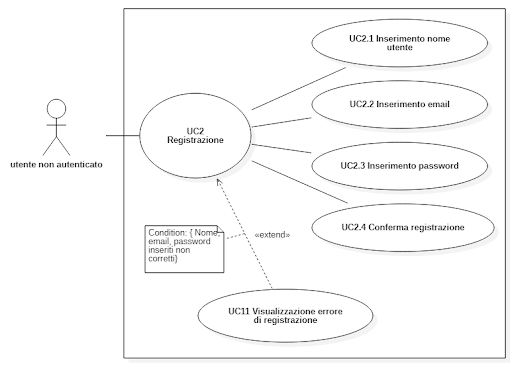
\includegraphics[width=1.0\textwidth]{res/images/esempio_caso_d_uso.png}
						\caption{Img.1 esempio caso d'uso}
						\label{fig:Img.1 esempio caso d'uso: UC2 Registrazione}
					\end{figure}
				\begin{itemize}
					\item\textbf{Attori}: Utente non autenticato;
					\item\textbf{Scopo e descrizione}: L’utente desidera registrarsi con un nuovo account inserendo dei dati personali;
					\item\textbf{Precondizione}: L’applicazione è stata avviata;
					\item\textbf{Flusso principale degli eventi:}
						\begin{enumerate}
							\item Inserimento nome utente (UC2.1)
							\item Inserimento email (UC2.2)
							\item Inserimento password (UC2.3)
							\item Conferma registrazione (UC2.4)
						\end{enumerate}
					\item\textbf{Scenari alternativi:}
						\begin{itemize}
							\item Se l’utente ha inserito dei dati non validi il sistema interrompe la fase di registrazione e mostra un errore (UC11 Visualizzazione errore di registrazione).
						\end{itemize}
					\item\textbf{Postcondizione}: L’utente inserendo e confermando i dati richiesti ha creato un nuovo account.
				\end{itemize}
			

		\subsubsection{Progettazione}
			\paragraph{Introduzione}
				\subparagraph{Descrizione}
					Il processo di Progettazione ha come risultato la realizzazione dell’architettura del sistema.\\
					Le due parti fondamentali sono:\\
					\begin{itemize}
						\item\textbf{technology baseline}: contiene le specifiche della progettazione ad alto livello del prodotto e delle sue componenti, l'elenco dei diagrammi UML che saranno utilizzati per la realizzazione dell'architettura e i test di verifica;
						\item\textbf{product baseline}: dettaglia ulteriormente l'attività di progettazione, integrando ciò che è riportato nella technology baseline. Inoltre definisce i test necessari alla verifica.
					\end{itemize}
				\subparagraph{Obbiettivi}
					Il processo di Progettazione, in risposta ai requisiti del documento “Analisi dei Requisiti”, individua le caratteristiche che il prodotto software richiesto deve possedere allo scopo di fornire la miglior soluzione adottabile per soddisfare i requisiti.\\
					É compito del Progettista svolgere tale attività attraverso la definizione logica del prodotto, identificando le varie componenti in modo chiaro, coeso e riutilizzabile in modo da rimanere dentro i costi fissati.\\
					L'architettura dovrà soddisfare i requisiti indicati nel documento “Analisi dei Requisiti”, adattandosi nel caso si evolvano o se ne aggiungano di nuovi. \\
					Deve rispettare le caratteristiche di comprensibilità, modularità e robustezza per garantire una riusabilità, ovvero un impiego delle sue parti anche in altre applicazioni. \\
					Inoltre si devono presentare componenti semplici, incapsulate, con un basso livello di accoppiamento e coese nel raggiungimento degli obiettivi per far sì che si abbia un impiego efficiente delle risorse necessarie.\\
					
		\subsubsection{Codifica}
			\paragraph{Introduzione}
				\subparagraph{Descrizione}
					La scrittura del codice dovrà rispettare quanto stabilito nella documentazione di prodotto. Dovrà perseguire gli obiettivi di qualità definiti all'interno del documento “Piano di Qualifica” per poter garantire una buona qualità del codice.\\
				\subparagraph{Obbiettivi}
					La codifica, svolta dal ruolo del Programmatore, ha come scopo quello di normare l’effettiva realizzazione del prodotto software richiesto, in modo che sia conforme alle richieste pressate con il Proponente. In questa fase si concretizza la soluzione trasformando in codice l’architettura ad alto livello pensata dai Progettisti rendendola eseguibile dai calcolatori.\\
					I Programmatori dovranno seguire queste norme durante le fasi di programmazione ed implementazione così da generare codice leggibile ed uniforme, agevolare le fasi di manutenzione, verifica e validazione e migliorare la qualità di prodotto.\\	

		\subsubsection{Metriche}
			La presente sezione espone le metriche selezionate dal gruppo per misurare il raggiungimento degli obiettivi di qualità del processo di Sviluppo. \\
			\paragraph{Completezza}
				Il prodotto finale deve essere il più possibile vicino a quello desiderato rispetto a efficienza, aspettative, utilizzo, vincoli rispettati e se il prodotto finale è conforme a quanto descritto nell’ ”Analisi dei Requisiti”. Per questo motivo si procederà a definire delle metriche che si baseranno su quanto descritto in tale documento.\\
				La valutazione delle conformità del prodotto finale ai requisiti richiesti verrà valutata tramite le seguenti metriche:\\
				\begin{itemize}
					\item\textbf{QM-PD-SVL01 Requisiti completati totali da piano di progetto fino a un determinato momento (RTOT)}
						\begin{itemize}
							\item\textbf{Descrizione}\\
								la metrica permette di conoscere il numero di requisiti conclusi in un determinato momento, con riferimento il \dext{Piano di Progetto}\\
							\item\textbf{Unità di misura}: intero
							\item\textbf{Formula}\\
								$$ \mathit{RTOT} = \sum_{r = \mathit{primo\;requisito}}^{\mathit{ultimo\;requisito}}
  									\begin{cases}
    										1       & \quad \text{se } r \text{ concluso in quel istante nel \dext{Piano di Progetto}}\\
    										0  & \quad \text{se } r \text{ altrimenti}
 								 	\end{cases}
								$$
							\item\textbf{Risultato}\\
								il numero di requisiti definiti da \dext{Piano di Progetto} che dovrebbero essere conclusi in un determinato momento
								\newline
								\newline
								\newline
						\end{itemize}
					\item\textbf{QM-PD-SVL02 Percentuale requisiti soddisfatti (PRS)}
						\begin{itemize}
							\item\textbf{Descrizione}\\
								la metrica permette di conoscere la percentuale dei requisiti di esposti nell’ “Analisi dei Requisiti” soddisfatti fino a quel momento, sulla base delle requisiti di qualità disponibili e espressi secondo metriche da noi definite;\\
							\item\textbf{Unità di misura}: percentuale
							\item\textbf{Formula}\\
								\[PRS = \frac{\mathit{\#requisiti\;\;soddisfatti}}{\mathit{RTOT}} \times 100 \]
							\item\textbf{Risultato}\\
								\begin{itemize}
									\item se il risultato è pari a 0\%, nessun requisito che dovrebbe esser soddisfatto, è stato soddisfatto.
									\item se il risultato è pari al 100\%, tutti i requisiti che dovrebbero esser soddisfatti,  sono stati soddisfatti.
									\item se il risultato è maggiore di 0\%, ma minore di 100\%, non tutti requisiti che dovrebbero esser soddisfatti, sono stati soddisfatti.
								\end{itemize}
						\end{itemize}
				\end{itemize}
		% rimosso per RR %
\iffalse
			\paragraph{Sicurezza}
			\paragraph{Affidabilità}
			\paragraph{Efficienza}
			\paragraph{Usabilità}
			\paragraph{Manutenibilità}
			\paragraph{Sviluppo}
\fi
	% fine rimossione %
	
		\subsubsection{Strumenti}
			\begin{itemize}
				\item\textbf{StarUML}: è un'applicazione online gratuita e collaborativa, per la realizzazione di diagrammi di molteplici tipologie. In particolare, risulta molto utile per la rappresentazione di diagrammi UML di qualsiasi tipologia, grazie ad un insieme di forme e figure in linguaggio UML predefinite all'interno dell'applicazione stessa e facilmente componibili per la costruzione dei diagrammi.
			\end{itemize}
			
			
			
			
			
			
			
			
			
			
			
			
			
			
			
\newpage		
				